\documentclass[a4paper,10pt]{article}
\usepackage[utf8]{inputenc}
\usepackage[T1]{fontenc}
\usepackage[sc]{mathpazo}
\usepackage[scaled=0.88]{helvet}
\usepackage{amsmath,amssymb,mathrsfs,stmaryrd}
\usepackage{microtype}
\usepackage[a4paper,top=1.5cm,bottom=1.5cm,left=1.4cm,right=1.4cm,headheight=12pt,headsep=0.4cm,footskip=0.7cm]{geometry}
\usepackage{xcolor}
\definecolor{Ink}{HTML}{1C2533}\definecolor{Bleu}{HTML}{1F3A5F}\definecolor{BleuMoyen}{HTML}{4A6A8F}
\definecolor{BleuClair}{HTML}{9DB2C9}\definecolor{Fond}{HTML}{F2F4F7}\definecolor{Ocre}{HTML}{B07A26}
\definecolor{Brique}{HTML}{A23B2A}\definecolor{Gris}{HTML}{5E6672}\definecolor{Filet}{HTML}{C5CCD6}
\usepackage{multicol,enumitem,booktabs,array,needspace}
\usepackage[most]{tcolorbox}
\usepackage{tikz,pgfplots}
\pgfplotsset{compat=1.17,trig format plots=rad}
\usetikzlibrary{arrows.meta}
\usepackage{fancyhdr}
\usepackage[colorlinks=true,linkcolor=Bleu,bookmarksopen=true,bookmarksopenlevel=0]{hyperref}

\setlength{\parindent}{0pt}\setlength{\parskip}{0.25em}
\setlength{\columnsep}{0.55cm}\setlength{\columnseprule}{0.3pt}\renewcommand{\columnseprulecolor}{\color{Filet}}
\setlist{itemsep=0.05em,topsep=0.15em,parsep=0pt,leftmargin=1.1em}
\setlist[itemize]{label=\textcolor{BleuMoyen}{\scriptsize\textbullet}}
\setlist[enumerate]{label=\textsf{\scriptsize\color{Bleu}\arabic*.},leftmargin=1.3em}
\linespread{1.02}

\newcommand{\K}{\mathbb{K}}\newcommand{\R}{\mathbb{R}}\newcommand{\C}{\mathbb{C}}\newcommand{\Z}{\mathbb{Z}}
\newcommand{\Mn}[1]{\mathcal{M}_{n}(#1)}\newcommand{\rg}{\operatorname{rg}}\newcommand{\vect}{\operatorname{Vect}}
\newcommand{\Mat}{\operatorname{Mat}}\newcommand{\Id}{\operatorname{Id}}\newcommand{\com}{\operatorname{com}}
\newcommand{\vv}[1]{\overrightarrow{#1}}\newcommand{\ve}[1]{\vec{#1}}
\newcommand{\dt}[1]{\left|\begin{matrix}#1\end{matrix}\right|}
\newcommand{\HP}{{\sffamily\bfseries\scriptsize\textcolor{Brique}{[HP]}}}
\newcommand{\livre}[1]{{\sffamily\scriptsize\color{Gris}[#1]}}

% ---------- titres ----------
\newcommand{\chapitre}[2]{\clearpage\phantomsection\pdfbookmark[0]{#1 --- #2}{chap#1}\markboth{#1 --- #2}{}%
  \noindent\colorbox{Bleu}{\parbox{\dimexpr\linewidth-2\fboxsep}{\color{white}\sffamily\bfseries\Large\strut #1\quad
  {\normalsize\mdseries #2}}}\par\vspace{0.4em}}
\newcommand{\notion}[1]{\par\needspace{9\baselineskip}\vspace{0.5em}\phantomsection\pdfbookmark[1]{#1}{\detokenize{#1}}\noindent{\sffamily\bfseries\color{Bleu}\large #1}\par\nobreak
  \noindent{\color{Ocre}\rule{\linewidth}{0.8pt}}\par\nobreak\vspace{0.1em}}
\newcommand{\sous}[1]{\par\needspace{6\baselineskip}\vspace{0.25em}\noindent{\sffamily\bfseries\small\color{BleuMoyen}#1}\par\nobreak}

% ---------- encadrés ----------
\tcbset{base/.style={enhanced,arc=0pt,boxrule=0pt,left=4pt,right=3pt,top=2pt,bottom=2pt,before skip=0.35em,after skip=0.35em,
  fontupper=\small}}
\newtcolorbox{DEF}[1][]{base,colback=white,borderline west={1.4pt}{0pt}{Bleu},
  before upper={{\sffamily\bfseries\scriptsize\color{Bleu}DÉFINITION\ifx\relax#1\relax\else\ --- #1\fi}\par}}
\newtcolorbox{PROP}[1][]{base,colback=Fond,borderline west={2pt}{0pt}{Bleu},
  before upper={{\sffamily\bfseries\scriptsize\color{Bleu}\ifx\relax#1\relax PROPRIÉTÉ\else #1\fi}\par}}
\newtcolorbox{FORM}[1][]{base,colback=white,colframe=BleuMoyen,boxrule=0.5pt,
  before upper={{\sffamily\bfseries\scriptsize\color{BleuMoyen}\ifx\relax#1\relax FORMULES\else #1\fi}\par}}
\newtcolorbox{METH}[1]{base,colback=white,borderline north={0.8pt}{0pt}{Bleu},borderline south={0.8pt}{0pt}{Bleu},
  before upper={{\sffamily\bfseries\scriptsize\colorbox{Bleu}{\color{white}MÉTHODE}\ \color{Bleu}#1}\par\smallskip}}
\newtcolorbox{PIEGE}{base,colback=Brique!5,borderline west={1.4pt}{0pt}{Brique},
  before upper={{\sffamily\bfseries\scriptsize\color{Brique}PIÈGES}\par}}
\newtcolorbox{ASTU}{base,colback=Ocre!7,borderline west={1.4pt}{0pt}{Ocre},
  before upper={{\sffamily\bfseries\scriptsize\color{Ocre}ASTUCES}\par}}
\newtcolorbox{HPBOX}{base,colback=white,borderline west={1.4pt}{0pt}{Brique},
  before upper={{\sffamily\bfseries\scriptsize\color{Brique}HORS PROGRAMME}\par}}

\pagestyle{fancy}\fancyhf{}
\fancyhead[L]{\scriptsize\sffamily\color{Gris}\leftmark}
\fancyhead[R]{\scriptsize\sffamily\scshape\color{Gris}Le Collé PT --- fiche Courbes paramétrées}
\fancyfoot[C]{\scriptsize\sffamily\thepage}
\renewcommand{\headrulewidth}{0.3pt}

\pgfplotsset{mini/.style={axis lines=middle,axis line style={Filet},xtick=\empty,ytick=\empty,width=3.2cm,height=3.2cm,
  xmin=-1.15,xmax=1.15,ymin=-1.15,ymax=1.15,title style={font=\scriptsize\sffamily,yshift=-0.15cm},samples=80}}

\begin{document}
\thispagestyle{empty}
\noindent\colorbox{Bleu}{\parbox{\dimexpr\linewidth-2\fboxsep}{\vspace{0.4em}
{\color{white}\sffamily\scriptsize\textls[200]{LE COLLÉ\ \ ·\ \ MATHÉMATIQUES PT\ \ ·\ \ CHAPITRE 2}}\par\smallskip
{\color{white}\sffamily\bfseries\LARGE Fiche de référence --- Courbes paramétrées planes}\par\smallskip
{\color{white!85!Bleu}\sffamily tangentes, plan d'étude, points stationnaires, branches infinies, tracé}\vspace{0.4em}}}

\vspace{0.6em}
{\small Le livre sert à apprendre, la présentation à comprendre, cette fiche à travailler et réviser. Elle reprend tout le cours du chapitre, les méthodes des exemples et les résultats des TD, avec les mêmes numéros de parties et les mêmes notations que la présentation. Les renvois \livre{§2.4} désignent les sections du livre ; \HP{} signale une notion hors programme utilisée en TD ou en devoir.}

\vspace{0.4em}
{\small\sffamily\noindent\begin{tabular}{@{}p{0.6\linewidth}@{}}
2.1 Fonctions vectorielles, outils de calcul \dotfill\pageref{n21}\\
2.2 Tangente, pente \dotfill\pageref{n22}\\
2.3 Plan d'étude, symétries, tracé \dotfill\pageref{n23}\\
2.4 Points stationnaires, inflexions \dotfill\pageref{n24}\\
2.5 Branches infinies, positions \dotfill\pageref{n25}\\
2.6 Intersections, points doubles \dotfill\pageref{n26}\\
2.7 Check-list et résultats des TD \dotfill\pageref{n27}\\
\end{tabular}}

\vspace{0.6em}
\pdfbookmark[0]{Chapitre 2 --- Courbes paramétrées planes}{chap2}\markboth{Chapitre 2 --- Courbes paramétrées planes}{}
\begin{multicols}{2}\raggedcolumns

\notion{2.1 Fonctions vectorielles, outils de calcul}\label{n21}

\begin{DEF}
Courbe paramétrée : $f:I\to\R^2$ (ou $\R^3$), $f(t)=\vv{OM(t)}=(x(t),y(t))$, de classe $\mathcal C^1$. Support
$\{M(t)\}$. Équation cartésienne $F(x,y)=0$ $\neq$ représentation paramétrique.\\
Droite $(AB)$ : $t\mapsto A+t\vv{AB}$. Cercle $(\Omega,R)$ : $\theta\mapsto\Omega+R(\cos\theta,\sin\theta)$. Graphe : $t\mapsto(t,g(t))$.
\end{DEF}

\begin{FORM}[DÉRIVATION]
Tout se lit sur les coordonnées : $f'=(x',y')$ vitesse, $f''$ accélération, $\|f'\|$ vitesse scalaire.\\
$(\lambda f+g)'=\lambda f'+g'$ ;\ $(\varphi f)'=\varphi'f+\varphi f'$ ;\ $(f\circ\varphi)'=\varphi'\,(f'\circ\varphi)$ ;\\
$(f\cdot g)'=f'\cdot g+f\cdot g'$ ;\ $(f\wedge g)'=f'\wedge g+f\wedge g'$ ($\R^3$) ;\\
Leibniz : $(\varphi f)^{(n)}=\sum\binom nk\varphi^{(k)}f^{(n-k)}$.\\
Taylor--Young : $f(t_0+h)=\sum_{k=0}^n\frac{h^k}{k!}f^{(k)}(t_0)+o(h^n)$.\\
$\|f\|$ constante $\Rightarrow f\cdot f'=0$.
\end{FORM}

\begin{FORM}[DÉVELOPPEMENTS LIMITÉS EN $0$ (rappels)]
$\frac1{1+u}=1-u+u^2-u^3+o(u^3)$\\
$\ln(1+u)=u-\frac{u^2}2+\frac{u^3}3+o(u^3)$\\
$e^u=1+u+\frac{u^2}2+\frac{u^3}6+o(u^3)$\\
$\sqrt{1+u}=1+\frac u2-\frac{u^2}8+\frac{u^3}{16}+o(u^3)$\\
$\cos u=1-\frac{u^2}2+\frac{u^4}{24}+o(u^5)$, $\sin u=u-\frac{u^3}6+\frac{u^5}{120}+o(u^6)$
\end{FORM}

\begin{METH}{Développer en $t_0\neq0$ ou à l'infini}
En $t_0$ : $t=t_0+h$, faire apparaître $1+u$ : $\frac1{-1+h}=-\frac1{1-h}$, $\ln(2+t)=\ln(1+h)$ si $t_0=-1$.\\
Inverse : écrire $e^t-1=t(1+u)$, puis $\frac1{1+u}$.\\
À l'infini : factoriser le terme dominant, $\ln(t+3)=\ln t+\ln(1+\frac3t)$, $e^{4/t}=1+\frac4t+\frac8{t^2}+\dots$\\
Même ordre pour $x$ et $y$ ; contrôler le terme constant.
\end{METH}

\begin{FORM}[TRIGONOMÉTRIE UTILE]
$1-\cos t=2\sin^2\frac t2$,\ $\sin t=2\sin\frac t2\cos\frac t2$,\ $\cos2t=2\cos^2t-1$.\\
$\cos3t=4\cos^3t-3\cos t$ ;\ $\sin3t=\sin t\,(4\cos^2t-1)$.\\
Angle moitié : $e^{ia}\pm e^{ib}=e^{i\frac{a+b}2}\big(e^{i\frac{a-b}2}\pm e^{-i\frac{a-b}2}\big)$ :\\
$\cos t-\cos2t=2\sin\frac t2\sin\frac{3t}2$ ;\ $\cos t+\cos2t=2\cos\frac t2\cos\frac{3t}2$ ;\\
$\sin t+\sin2t=2\cos\frac t2\sin\frac{3t}2$.\\
Linéariser : $\sin a\sin b=\frac{\cos(a-b)-\cos(a+b)}2$, $\cos a\cos b=\frac{\cos(a-b)+\cos(a+b)}2$.
\end{FORM}

% ======================================================================
\notion{2.2 Tangente, pente}\label{n22}

\begin{DEF}
$M(t_0)$ \emph{régulier} si $f'(t_0)\neq\ve0$, \emph{stationnaire} sinon ; courbe régulière : tous ses points réguliers.
Tangente = limite des droites $M(t_0)+\vect(\ve u_h)$, $\ve u_h$ unitaire dirigeant la corde $[M(t_0)M(t_0+h)]$.
Orientation : sens de parcours, ou $\frac{f'}{\|f'\|}$.
\end{DEF}

\begin{PROP}[TANGENTE EN UN POINT RÉGULIER \livre{th.~2.3}]
$T=M(t_0)+\vect f'(t_0)$ ; équation
\[\det\big(\vv{M(t_0)M},f'(t_0)\big)=0\iff y'_0(x-x_0)-x'_0(y-y_0)=0.\]
Horizontale $\iff y'(t_0)=0$ ; verticale $\iff x'(t_0)=0$ (point régulier !).\\
Pente $p=\frac{y'}{x'}$ si $x'\neq0$ (car $y=g(x)$ localement, $y'=g'(x)x'$).\\
Parallèle à $\ve w$ : $\det(f',\ve w)=0$ ; pente $m$ : $y'=m\,x'$.
\end{PROP}

\begin{PIEGE}
« $x'=0$ donc verticale » : faux si $y'=0$ aussi (point stationnaire).\\
$\frac yx$ = pente de $(OM)$, pas de la tangente ; égalité seulement à la limite $M(t)\to O$.\\
Tangente de pente $m$ : simplifier $\frac{y'}{x'}$ avant de résoudre ; vérifier la régularité.
\end{PIEGE}

% ======================================================================
\notion{2.3 Plan d'étude, symétries, tracé}\label{n23}

\begin{METH}{Étudier une courbe \livre{méth.~2.1}}
\begin{enumerate}
\item Domaine ; valeurs interdites et bornes (branches).
\item Réduction : période, puis symétries (tableau).
\item $x'$, $y'$ \emph{factorisées} (même dénominateur) : stationnaires = zéros communs ; tangentes horizontales/verticales.
\item Tableau conjoint, valeurs, limites.
\item Stationnaires (§2.4), branches (§2.5), inflexions, points doubles.
\item Tracé (ci-dessous).
\end{enumerate}
\end{METH}

\begin{FORM}[SYMÉTRIES : chercher $\varphi$ avec $M(\varphi(t))=s(M(t))$]
\renewcommand{\arraystretch}{1.1}
\begin{tabular}{@{}lll@{}}
$f(-t)=(x,-y)$ & axe $(Ox)$ & $t\geq0$\\
$f(-t)=(-x,y)$ & axe $(Oy)$ & $t\geq0$\\
$f(-t)=-f(t)$ & centre $O$ & $t\geq0$\\
$f(\frac1t)=(y,x)$ & axe $y=x$ & $|t|\leq1$\\
$f(\pi-t)=(\pm x,\pm y)$ & selon signes & demi-intervalle\\
$f(t+T)=f(t)$ & période & une période
\end{tabular}\\
Compléter dans l'ordre inverse des réductions.
\end{FORM}

\begin{ASTU}
Point sur un axe de symétrie : tangente $\perp$ à l'axe (point de raccord), sauf point stationnaire ou double.\\
Vérifier qu'une symétrie supposée est compatible ($f$ impaire $\Rightarrow f(0)=O$ ; période $T$ $\Rightarrow f(0)=f(T)$).\\
$t\mapsto\frac1t$ transforme les branches $t\to\infty$ en branches $t\to0$.
\end{ASTU}

\begin{METH}{Tracer \livre{fiche §2.7}}
Asymptotes en pointillés ; points nommés avec un segment de tangente ; arcs selon le tableau : signes de $(x',y')$ :
$(+,+)$ haut-droite, $(+,-)$ bas-droite, $(-,+)$ haut-gauche, $(-,-)$ bas-gauche ; positions par rapport aux asymptotes et
tangentes ; symétries ; flèches de sens.
\end{METH}

% ======================================================================
\notion{2.4 Points stationnaires, étude locale, inflexions}\label{n24}

\begin{DEF}[NATURE D'UN POINT]
\emph{Ordinaire} : la courbe reste du même côté de sa tangente. \emph{Inflexion} : elle la traverse. \emph{Rebroussement} : elle
s'arrête et repart en arrière, en traversant sa tangente (1\textsuperscript{re} espèce) ou non (2\textsuperscript{e} espèce).
\emph{Anguleux} : deux demi-tangentes non colinéaires ($(t,|t|)$ en $0$).
\end{DEF}

\begin{PROP}[THÉORÈME $(p,q)$ \livre{th.~2.5}]
$p=\min\{k\geq1:f^{(k)}(t_0)\neq\ve0\}$, $q=\min\{k>p:(f^{(p)},f^{(k)})\text{ libre}\}$. Tangente dirigée par $f^{(p)}(t_0)$.\\[2pt]
\begin{tabular}{@{}c|cc@{}}
 & $q$ pair & $q$ impair\\\hline
$p$ impair & ordinaire & inflexion\\
$p$ pair & rebr. 2\textsuperscript{e} esp. & rebr. 1\textsuperscript{re} esp.
\end{tabular}\\[2pt]
Raison : dans $(M_0,f^{(p)},f^{(q)})$, $X\sim\frac{h^p}{p!}$, $Y\sim\frac{h^q}{q!}$ ; $p$ impair : $X$ change de signe ; $q$
impair : la courbe traverse sa tangente.
\end{PROP}

\begin{center}
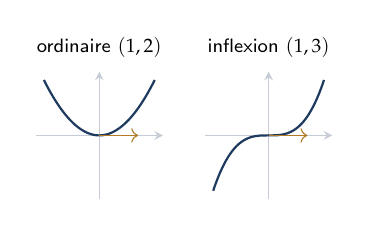
\begin{tikzpicture}
\begin{axis}[mini,title={ordinaire $(1,2)$}]\addplot[Bleu,thick,domain=-1:1]({x},{x^2});\draw[Ocre,->](axis cs:0,0)--(axis cs:0.7,0);\end{axis}
\begin{axis}[mini,xshift=2.15cm,title={inflexion $(1,3)$}]\addplot[Bleu,thick,domain=-1:1]({x},{x^3});\draw[Ocre,->](axis cs:0,0)--(axis cs:0.7,0);\end{axis}
\end{tikzpicture}\\
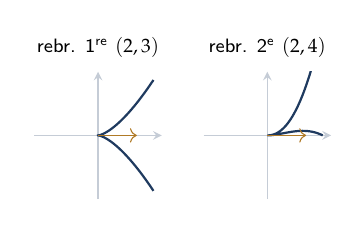
\begin{tikzpicture}
\begin{axis}[mini,title={rebr. 1\textsuperscript{re} $(2,3)$}]\addplot[Bleu,thick,domain=-1:1]({x^2},{x^3});\draw[Ocre,->](axis cs:0,0)--(axis cs:0.7,0);\end{axis}
\begin{axis}[mini,xshift=2.15cm,title={rebr. 2\textsuperscript{e} $(2,4)$}]\addplot[Bleu,thick,domain=-1:1]({x^2},{x^4+x^5});\draw[Ocre,->](axis cs:0,0)--(axis cs:0.7,0);\end{axis}
\end{tikzpicture}
\end{center}

\begin{METH}{Point stationnaire par DL \livre{méth.~2.2}}
\begin{enumerate}
\item $t=t_0+h$ ; DL de $x$ et $y$.
\item $f(t_0+h)=f(t_0)+h^p\ve a+\dots+h^q\ve b+o(h^q)$ ; s'arrêter au premier $\ve b$ avec $\det(\ve a,\ve b)\neq0$.
\item Tangente : $M_0+\vect\ve a$, équation $\det(\vv{M_0M},\ve a)=0$ (\emph{pas} $f'(t_0)=\ve0$).
\item Position : du côté de $\ve b$ quand $h^q>0$ ; ou $\varphi=\alpha x+\beta y+\gamma\sim ch^q$ pour la tangente $\alpha x+\beta y+\gamma=0$.
\end{enumerate}
\end{METH}

\begin{PIEGE}
Terme intermédiaire colinéaire au premier : il ne compte pas. Terme nul : aller plus loin (ordre 4 ou 5, TD~7).\\
Stationnaire $\not\Rightarrow$ rebroussement : $(t^3,t^5)$ inflexion, $(t^3,t^4)$ ordinaire.\\
Point anguleux : demi-tangentes non colinéaires ($f'$ discontinue, $(t,|t|)$).
\end{PIEGE}

\begin{FORM}[INFLEXION ET $\det(f',f'')$ \livre{§2.4}]
Si $x'\neq0$ : $y(t)=g(x(t))$ et
\[g''(x(t))=\frac{x'y''-y'x''}{x'^3}=\frac{\det(f',f'')}{x'^3}.\]
Inflexion (point régulier) $\iff\det(f',f'')$ \emph{change de signe}. Nécessaire : $\det=0$.\\
Birégulier ($\det\neq0$) : point ordinaire, courbe du côté de $f''$.\\
Pente : $p'=\frac{\det(f',f'')}{x'^2}$ $\Rightarrow$ pente extrémale à l'inflexion (racine double de $p(t)=m$).\\
Si $x'=0$ : $x=h(y)$, $h''=-\frac{\det(f',f'')}{y'^3}$.
\end{FORM}

\begin{METH}{Chercher les inflexions \livre{méth.~2.3}}
\begin{enumerate}
\item Factoriser la vitesse : $f'=\lambda\ve g$, $\lambda$ scalaire $\neq0$ $\Rightarrow$ $\det(f',f'')=\lambda^2\det(\ve g,\ve g')$.
\item Résoudre $\det(\ve g,\ve g')=0$ aux points réguliers ; trigonométrique : linéariser.
\item Confirmer : changement de signe, ou $\det(f',f''')\neq0$ ($q=3$). Stationnaires : par DL ($p,q$ impairs).
\end{enumerate}
Piège : c'est la colinéarité $f''\parallel f'$ qui compte, pas $f''=\ve0$ ($(t+t^2,t^3)$ : inflexion avec $f''(0)\neq\ve0$ ;
$(t,t^4)$ : $f''(0)=\ve0$, pas d'inflexion).
\end{METH}

% ======================================================================
\notion{2.5 Branches infinies, positions}\label{n25}

\begin{DEF}
$\|\vv{OM}\|\to\infty$ quand $t\to t_0$ : $\mathcal D$ asymptote si $d(M(t),\mathcal D)\to0$.\\
$d(M_0,ax+by+c=0)=\frac{|ax_0+by_0+c|}{\sqrt{a^2+b^2}}$.
\end{DEF}

\begin{METH}{Classer une branche \livre{méth.~2.4}}
Pour \emph{chaque} borne et valeur interdite :
\begin{enumerate}
\item $x\to\pm\infty$, $y\to b$ : $y=b$ ; $x\to a$, $y\to\pm\infty$ : $x=a$.
\item $x,y$ infinis : $\frac yx\to\infty$ : branche parab.\ $(Oy)$ ; $\to0$ : $(Ox)$ ; $\to\alpha\neq0$ : calculer $\lim(y-\alpha x)$ ;
      $=\beta$ : asymptote $y=\alpha x+\beta$ ; infinie : branche parab.\ de direction $y=\alpha x$.
\item Position : signe de $y-\alpha x-\beta$ (développement asymptotique, ou monotonie).
\item $x,y$ finis : point limite $A$ ; tangente : $\lim\frac{y-y_A}{x-x_A}$ ; cercle creux s'il n'est pas atteint.
\end{enumerate}
\end{METH}

\begin{METH}{Position globale par rapport à une droite \livre{méth.~2.5}}
$\varphi(t)=ax(t)+by(t)+c$ : zéros = intersections ; signe = côté ($b<0$ : $\varphi>0$ signifie au-dessous).
Étudier $\varphi$ (dérivée factorisée, tableau). Tangente en $M(t_0)$ : $t_0$ racine double de $\varphi$, donc $(t-t_0)$ facteur de
$\varphi'$.
\end{METH}

\begin{PIEGE}
$\lim\frac yx$ seul ne prouve pas l'asymptote. Oublier une borne du domaine ($t\to-2$, $t\to-3$\dots).\\
Factoriser le dénominateur ($1+t^3=(1+t)(1-t+t^2)$) avant de calculer $y-\alpha x$.\\
Carré au numérateur de $y-\alpha x-\beta$ : même côté des deux côtés.
\end{PIEGE}

\begin{HPBOX}
\textbf{Courbe asymptote} $\Gamma$ : exhiber $P_t\in\Gamma$ avec $M(t)P_t\to0$. Même abscisse : $y-g(x)\to0$ (parabole :
$y-\frac{x^2}2\to0$). Même ordonnée pour une exponentielle : $x-\ln(y-c)\to0$, vrai pour \emph{toute} constante $c$ ; seule la
distance verticale en privilégie une.\\
\textbf{Polaires} : $x=r\cos\theta$, $y=r\sin\theta$, partir de $x^2+y^2=r^2$. Cardioïde $r=1-\cos\theta$ ; lemniscate
$(x^2+y^2)^2=xy$, $r^2=\frac12\sin2\theta$.
\end{HPBOX}

% ======================================================================
\notion{2.6 Intersections, points doubles}\label{n26}

\begin{METH}{Intersection courbe/droite}
Substituer $x(t)$, $y(t)$ dans l'équation de la droite. Trigonométrique : tout en $X=\cos t$, élever au carré ($\sin^2t=1-X^2$),
factoriser ; \emph{vérifier les signes} à la fin. Tangence : racine double ; autre branche par le même point : racine de plus.
\end{METH}

\begin{METH}{Points doubles}
Résoudre $f(t)=f(s)$, $t\neq s$ ; une symétrie aide (point de l'axe $(Oy)$ : $x(t)=0$). Sans formule (tableau) : écrire deux arcs
comme graphes ($x$ monotone) et appliquer le TVI à $h_1-h_2$, avec les pentes aux extrémités \livre{TD~1}.
Tangentes au point double : une par paramètre.
\end{METH}

\begin{ASTU}
Lissajous $(\cos3t,2\sin t)$ \livre{§2.6} : point double $J=(0,1)$ ($t=\frac\pi6,\frac{5\pi}6$), tangentes $y=\mp\frac x{\sqrt3}+1$ ;
$T_2$ recoupe la courbe en $K\approx(0{,}62\,;1{,}36)$ (élévation au carré, signe vérifié) ; inflexion : linéariser,
$\det=12\cos2t+6\cos4t$, $\cos2\alpha=\frac{\sqrt3-1}2$, $\alpha\approx0{,}598$, quatre inflexions.
\end{ASTU}

% ======================================================================
\notion{2.7 Check-list et résultats des TD}\label{n27}

\begin{METH}{Check-list d'une étude}
\begin{enumerate}
\item Domaine, valeurs interdites ; symétries vérifiées.
\item Dérivées factorisées ; zéros communs.
\item Tangentes : régularité vérifiée.
\item DL jusqu'au premier vecteur non colinéaire.
\item Toutes les branches ; $\lim(y-\alpha x)$ ; position.
\item Position globale : $\varphi$ ; inflexions : $\lambda\ve g$.
\item Élévation au carré : signes.
\item Tracé fidèle (positions, tangentes, symétries).
\end{enumerate}
\end{METH}

{\small
\renewcommand{\arraystretch}{1.12}
\begin{tabular}{@{}>{\sffamily\scriptsize\bfseries\color{Bleu}}l>{\raggedright\arraybackslash}p{0.84\linewidth}@{}}
TD1 & Tangente en $\frac{5\pi}6$ : $x-4y+10=0$ ; $g$ non injective (TVI, point double) ; $\pi$-périodicité incompatible.\\
TD2 & $M=(a\cos\theta,b\sin\theta)$ ; tangence $\tan\theta=\sqrt{b/a}$ ($a=2,b=1$ : $35{,}3^\circ$).\\
TD3 & Axe $(Oy)$, période $\pi$ ; $T$ en $\frac\pi4$ : $x-2y+a=0$ ; $O$ rebr.\ 1\textsuperscript{re} esp.\ tangente $(Oy)$ ; asymptote
      $y=2a$ (dessous) ; $x^2(2a-y)=y^3$ ; construction : $\vv{OP}=\vv{QH}$ avec $OQ=2a\cos\theta$, $OH=\frac{2a}{\cos\theta}$.\\
TD4 & Axe $(Ox)$ ; $x'=\sin t(2\cos t-1)$, $y'=2\sin\frac t2\sin\frac{3t}2$ ; $O$ rebr.\ 1\textsuperscript{re} esp.\ tangente $(Ox)$ ;
      longueur $8$.\\
TD5 & $M(\frac1t)$ symétrique par $y=x$ ; $f$ impaire ; $O$ double (tangentes $(Ox)$, $(Oy)$) ; $(x^2+y^2)^2=xy$.\\
TD6 & $\det=-\frac32(t-2)(t+2)$ : inflexions $O$ (tangente $x=0$) et $(-16,0)$ (tangente $y=-\frac13(x+16)$) ; branches
      paraboliques $(Ox)$.\\
TD7 & En $\frac\pi2$ : $h^2(-\frac12,\frac12)+h^4(\frac1{24},-\frac16)$ : rebr.\ 2\textsuperscript{e} esp., tangente $x+y=1$ ;
      $A\approx(0{,}81;0{,}10)$.\\
TD8 & Symétrie $y=x$ ; asymptote $y=-x-\frac13$, courbe au-dessus ($\frac{(t+1)^2}{3(t^2-t+1)}>0$).\\
TD9 & $M(1)=(\frac32,\frac32)$ rebr.\ 1\textsuperscript{re} esp.\ tangente $y=x$ ; parabole asymptote $y=\frac{x^2}2$
      ($y-\frac{x^2}2\sim\frac1{2t}$) ; symétrie $y=x$.\\
TD10 & Asymptote $y=x-\frac12$ (dessus si $t\to0^+$) ; points limites $O$ et $(0,-1)$, tangentes horizontales.
\end{tabular}}

\end{multicols}
\end{document}
